\section{Algoritmer med faste parametre}%
\label{sec:algoparametre}

\begin{frame}
  \frametitle{Pensum}
  \begin{itemize}
    \item Cygan et al pp. 3-8, 12-14, 17--22, 51-55: \textbf{Algoritmer med faste parametre}.
    \item F.V. Fomin, D. Kratsch pp. 1-6: \textbf{Eksakte Algoritmer}.
    \item Weekly Note 13
    \item Video 26
  \end{itemize}
\end{frame}

\begin{frame}{Introduktion}
    Antag at du er ejer af en bar. Du skal sørge for at der ikke kommer nogen slåskampe.
    \begin{itemize}
        \item Du kender allerede de personer der gerne vil slås, og hvem de gerne vil slås med.
        \item Dit mål er derfor at, givet $n$ personer, vil du gerne ekskludere $k$ personer, således at så få personer som muligt kommer op og slås.
    \end{itemize}
\end{frame}

\begin{frame}{Vertex-Cover Problem}
    \begin{itemize}
        \item Vi kan modellere dette som et problem af \textsc{Vertex-Cover} problemet.
        \item Her er en knude en person, og en kant mellem to knuder betyder at de to knuder vil slås.
    \end{itemize}
\end{frame}

\begin{frame}{Eksempel på en graf}
    \begin{figure}
        \centering
        \begin{tikzpicture}[scale=0.5]
            \begin{scope}[every node/.style={circle,thick,draw}]
                \node (A) at (0,0) {};
                \node (B) at (0,3) {};
                \node (C) at (2.5,4) {};
                \node (D) at (2.5,1) {};
                \node (E) at (2.5,-1) {};
                \node (F) at (5,2) {};
            \end{scope}
            \begin{scope}[>={Stealth[black]}]
                \path [-] (A) edge node {} (B);
                \path [-] (A) edge node {} (D);
                \path [-] (D) edge node {} (C);
                \path [-] (D) edge node {} (E);
                \path [-] (D) edge node {} (F);
                \path [-] (E) edge node {} (F);
            \end{scope}
        \end{tikzpicture}
        \caption{\label{fig:barfightvertexcover} En graf $G = (V,E)$.}
    \end{figure}
    \begin{itemize}
        \item I Figur~\ref{fig:barfightvertexcover} ses et eksempel på en normal graf.
        \item Hver knude en person, og hver kant mellem to knuder, en slåskamp der venter på at ske.
    \end{itemize}
\end{frame}

\begin{frame}{Barkampsproblemet}
    \begin{itemize}
        \item Vi skal løse barkampsproblemet, men da \textsc{Vertex-Cover} er $\mathcal{NP}$-komplet, kan vi ikke bare gøre det som normalt.
        \item Der er to umiddelbare metoder: \textit{Den Naive Metode} og \textit{Binomialmetoden}.
    \end{itemize}
\end{frame}

\begin{frame}{Naive og Binomialmetoder}
    \begin{itemize}
        \item Naive Metode: Prøver alle $2^{1000} \approx 1.07 \cdot 10^{301}$ delmængder.
        \item Binomialmetoden: Prøver alle $\binom{n}{k}$ delmængder af størrelse $k$, hvilket er cirka $2.63 \cdot 10^{23}$ muligheder.
    \end{itemize}
\end{frame}

\begin{frame}{Problemreducering og Kernelisering}
    \begin{itemize}
        \item Vores løsning til problemet er at tage instansen og give det nogle regler, som vi kalder "sikkerhedsregler".
        \item Disse regler sikrer et mindre input, som vi så kan arbejde med.
    \end{itemize}
\end{frame}

\begin{frame}{Regler for Vertex-Cover}
    Givet en graf $G = (V,E)$ og et ikke-negativt heltal $k$:
    \begin{itemize}
        \item \textbf{Regel 1}: Hvis $\forall v \in V \mid d(v) = 0$, så fjerner vi $v$ fra grafen.
        \item \textbf{Regel 2}: Hvis $\forall v \in V \mid d(v) \ge k + 1$ så fjerner vi $v$ og reducerer $k$ med én.
        \item \textbf{Regel 3}: Hvis $\forall v \in V \mid d(v) = 1 \text{ og } w \text{ er den eneste nabo til }v$ så fjerner vi $v$ og $w$ i grafen, og reducerer $k$ med 1.
    \end{itemize}
\end{frame}

\begin{frame}{Reduktion og Kernelisering}
    \begin{itemize}
        \item Vi putter disse regler på inputtet $G$ indtil ingen af dem er mulige længere.
        \item Hvis $k' = 0$ og der stadig er kanter i grafen, så kan vi afvise $(G, k)$.
    \end{itemize}
\end{frame}

\begin{frame}{Eksempel på Kernelisering}
    \begin{itemize}
        \item Hvis $|E'| \le k'^{2}$ og $|V(G')| \le k^{2}$.
        \item Vi får dette resultat fra følgende udregning:
    \end{itemize}
    \begin{equation*}
        |V'| = \sum_{v \in V'} 1 = \frac{1}{2} \sum_{v \in V'} 2 \le \frac{1}{2} \sum_{v \in V'} d(v) = |E'| \le k'^{2} \le k^{2}
    \end{equation*}
\end{frame}

\begin{frame}{Brute-Force Algoritme}
    \begin{itemize}
        \item Når vi har sat disse regler ind og udført dem, kan vi køre en brute-force algoritme på inputtet $(G', k')$.
        \item Hvis $k = 10$ betyder det at vi højest skal prøve $\binom{100}{10} \approx 1.73 \cdot 10^{13}$ mulige delmængder.
    \end{itemize}
\end{frame}

\begin{frame}{Tid på Kernelisering}
    \begin{itemize}
        \item Tiden der bliver brugt i kerneliseringen af inputtet er $O((n+m)k)$.
        \item Hvis vi ikke afviser instansen, så kommer vi til en instans $(G', k')$.
    \end{itemize}
\end{frame}

\begin{frame}{Definitioner}
    \begin{itemize}
        \item \textbf{Parameteriseret Problem}: Et \textit{parameteriseret problem} $Q$ er \textit{Fastsat Parameter Traktabel} (FPT) hvis der eksisterer en algoritme $A_{Q}$ der løser $Q$ i tid $O(f(k) \cdot n^{c})$ for en beregnlig funktion $f$ og en konstant $c \in \mathbb{R}_{+}$.
        \item \textbf{Kernelisation, kernel}: En kernelisationsalgoritme (en kernel) for et parameteriseret problem $Q$ er en algoritme $A_{Q}$, som, givet en instans $(I,k)$ kører i polynomiel tid i $|(I,k)|$ og outputter en ækvivalent instans $(I', k')$, hvor $|I'| + k' \le g(k)$ for hver instans $(I, k)$ af $Q$ og $g$ er en fastsat beregnelig funktion.
    \end{itemize}
\end{frame}

\begin{frame}{Kernel til Vertex-Cover}
    \begin{itemize}
        \item Ved \textsc{Vertex-Cover} problemet, tog vi input $(G, k)$ og producerede en kernel $(G', k')$ som opfylder kravet $|G'| + k' \le 2k^{2} + k$.
    \end{itemize}
\end{frame}

\begin{frame}{En kernel af størrelse højest $2k$ til \textsc{Vertex-Cover}}
    \begin{itemize}
        \item I delkapitel så vi den følgende approximationsalgoritme baseret på lineær programmering for \textsc{Vertex-Cover}.
    \end{itemize}
    \begin{enumerate}
        \item Løs $Z_{LP} = \min \sum_{v \in V} X(v)$ således at $X(u)+X(v) \ge 1 \; \forall (u,v) \in E$ og $0 \le X(u) \le 1$.
        \item Lad $\hat{X}$ være en optimal LP-løsning.
        \item Tag $U = \{v \mid \hat{X}(v) \ge \frac{1}{2}\}$
    \end{enumerate}
\end{frame}

\begin{frame}{Nemhauser-Trotter Sætning}
    \begin{itemize}
        \item Der eksisterer et optimalt vertex-cover $U^{*}$ således at $V_{>} \subseteq U^{*} \subseteq V_{=} \cup V_{>}$.
        \item Bevis: Antag at $X$ er et optimal vertex-cover af $G = (V,E)$ og at $X \cap V_{<} \ne \emptyset$.
    \end{itemize}
\end{frame}

\begin{frame}{Lad $k^{*} = |U^{*}|$}
    \begin{itemize}
        \item Husk at vi kan antage at $V_{>} \subseteq U^{*}$.
        \item Lad $G' $ være delgrafen af $V_{=}$, og lad $k' = k - |V_{>}|$.
    \end{itemize}
\end{frame}

\begin{frame}{Tilbage til Barkampsanalogien}
    \begin{itemize}
        \item Først løser vi det lineære programmeringsproblem.
        \item Så finder vi $V_{<}, V_{=}$ og $V_{>}$.
        \item Hvis $|V_{>}| \ge k$ afviser vi.
    \end{itemize}
\end{frame}

\begin{frame}{Træsøgning}
    \begin{itemize}
        \item Vi vil nu vise hvordan man kan løse bedre end brute-force.
        \item Givet en instans $(G,k)$, prøv kanterne i en eller anden ordning.
    \end{itemize}
    \begin{figure}
        \centering
        \begin{tikzpicture}[level distance=1.5cm,
                level 1/.style={sibling distance=3cm},
                level 2/.style={sibling distance=1.5cm}]
            \node {a-b}
            child {node {b-c}
                    child {node {c-d}}
                    child {node {b-d}}
                }
            child {node {c-d}
                    child {node {d-e}}
                    child {node {e-f}}
                };
        \end{tikzpicture}
        \caption{\label{fig:treesearchvc} Træsøgning til \textsc{Vertex-Cover}}
    \end{figure}
\end{frame}

\begin{frame}{Eksempel på en graf}
    \begin{figure}
        \centering
        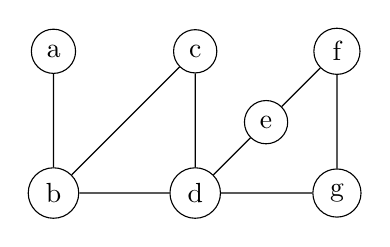
\begin{tikzpicture}
            [scale=1.8,every node/.style={circle,draw=black}]
            \node (a) at (1,2) {a};
            \node (b) at (1,1)  {b};
            \node (c) at (2,2)  {c};
            \node (d) at (2,1) {d};
            \node (e) at (2.5,1.5)  {e};
            \node (f) at (3,2)  {f};
            \node (g) at (3,1)  {g};

            \foreach \from/\to in {a/b, b/c, c/d, b/d, d/e, d/g, e/f, g/f} \draw (\from) -- (\to);
        \end{tikzpicture}
        \caption{\label{fig:treegraph} Grafen tilhørende træet.}
    \end{figure}
    \begin{itemize}
        \item I Figur~\ref{fig:treegraph} ses et eksempel på en graf hvor vertex coveret fundet ved hjælp af træsøgningsalgoritmen bliver $\{b,d,f\}$.
    \end{itemize}
\end{frame}

\begin{frame}{Køretid}
    \begin{itemize}
        \item Størrelsen af træet er højest $k-1$ og dybden er $k$, dermed er der højest $2^{k}-1$ delproblemer.
        \item Vi får fra regel 2 i vores kernelisering at hvis $d(v) \ge k+1$ skal den ud.
    \end{itemize}
\end{frame}

\section{Eksakte Algoritmer}

\begin{frame}{Kilder}
    \begin{itemize}
        \item Video 26
    \end{itemize}
\end{frame}

\begin{frame}{Eksponentiel tid}
    \begin{theorem}
        Hvert problem i $\mathcal{NP}$ kan løses i eksponentiel tid.
    \end{theorem}
    \begin{itemize}
        \item Bevis: Lad $L$ være et problem i $\mathcal{NP}$, og lad $p(k)$ være et polynomium.
        \item $x \in L$ hvis og kun hvis der findes en streng $y = y(x)$ af længde højst $p(|x|)$.
    \end{itemize}
\end{frame}

\begin{frame}{Ny Notation}
    \begin{itemize}
        \item Vi definerer ny en ny notation, $O^{*}$ til at være asymptotisk $O$-notation, men hvor vi ignorerer de polynomielle faktorer.
        \item $O(n^{3}\log^{2}n 3^{n/2}) = O^{*}(3^{n/2})$.
    \end{itemize}
\end{frame}

\begin{frame}{Optimal Løsning til \textsc{Vertex-Cover}}
    \begin{itemize}
        \item Husk træsøgningen for \textsc{Vertex-Cover} problemet.
        \item Der bruge vi et træ til at finde en dækning af størrelse $k$.
    \end{itemize}
    \begin{figure}
        \centering
        \begin{tikzpicture}[
            level 1/.style={sibling distance=6cm},
            level 2/.style={sibling distance=3cm},
            level 3/.style={sibling distance=1.5cm},
            edge from parent/.style={draw, -{Latex}},
            edge from parent path={(\tikzparentnode) -- (\tikzchildnode)},
            scale=0.6
            ]

            % Root
            \node {$\circ$}
            child {node {$\circ$}
                    child {node {$\circ$}
                            child {node {$\circ$}}
                            child {node {$\circ$}}
                        }
                    child {node {$\circ$}
                            child{node {$\circ$}}
                            child{node {$\circ$}}
                        }
                }
            child {node {$\circ$}
                    child {node {$\circ$}
                            child{node {$\circ$}}
                            child{node {$\circ$}}
                        }
                    child {node {$\circ$}
                            child {node {$\circ$}}
                            child {node {$\circ$}}
                        }
                };

            % Labels
            \node[right] at (2,-0.5) {$v_1$};
            \node[right] at (4,-2.0) {$v_2$};
            \node[right] at (5,-3.5) {$v_3$};

            % Set X
            \node[below right] at (4.5,-4.5) {$X = \{v_1, v_2, v_3\}$};

            % Initial X
            \node[left] at (-4.5,-5.0) {$X = \emptyset$};

        \end{tikzpicture}
        \caption{\label{fig:treesearchoptimal} Træsøgning til optimal dækning.}
    \end{figure}

\end{frame}

\begin{frame}{Antal Blade i Søgetræ}
    \begin{itemize}
        \item Vi kan begrænse arbejdet vi laver ved at kigge på antallet af blade i et binært søgetræ.
        \item Lad $T(n)$ være antallet af blade i søgetræet for grafer på $n$ knuder.
    \end{itemize}
    \begin{equation*}
        T(n) \le T(n-1) + T(n-1)
    \end{equation*}
\end{frame}

\begin{frame}{Bedre Algoritme}
    \begin{itemize}
        \item Gå deltræet igennem på en klog måde.
        \item Brug problemspecifikke observationer til at reducere antallet af blade i søgetræet.
    \end{itemize}
\end{frame}

\begin{frame}{Bedre Grænse}
    \begin{itemize}
        \item Hvis vi afviser $v$, skal vi inkludere mindst 3 knuder i dækningen.
        \item Dermed får vi grænsen:
    \end{itemize}
    \begin{equation*}
        T(n) \le T(n-1) + T(n-4)
    \end{equation*}
\end{frame}

\begin{frame}{Eksakt Algoritme til \textsc{Traveling-Salesman-Problem}}
    \begin{itemize}
        \item Givet $n$ knuder, $v_{1}, v_{2}, \ldots, v_{n}$ og deres distancer $d(v_{i}, v_{j}) \; \forall i \ne j$.
        \item Vi søger en permutation \(\Pi\) af $\{1,2, \ldots, n\}$.
    \end{itemize}
    \begin{equation}
        m = d(v_{\Pi(n)}, v_{\Pi(i)}) + \sum_{i=1}^{n-1}  d(v_{\Pi(i)}, v_{\Pi(i+1)})
    \end{equation}
\end{frame}

\begin{frame}{Optimal Løsning med Dynamisk Programmering}
    \begin{itemize}
        \item For hver delmængde $S \subseteq \{v_{2}, v_{3}, \ldots v_{n}\}$ og $v_{i} \in S$, lad $OPT[S, v_{i}]$ være længden af den korteste vej som starter i $v_{1}$.
    \end{itemize}
\end{frame}

\begin{frame}{Dynamisk Programmering}
    \begin{lemma}
        \begin{equation*}
            OPT[S, v_{i}] =
            \begin{cases}
                d(v_{1}, v_{i}) & \text{ hvis } S=\{v_{i}\} \\
                \min\{OPT[S-{v_{i}},v_{k}]+d(v_{k},v_{i}) \mid v_{k} \in S-{v_{i}}\} & \text{ hvis} \{v_{i}\} \subset S
            \end{cases}
        \end{equation*}
    \end{lemma}
\end{frame}

\begin{frame}{Algoritme}
    \begin{algorithm}
        \caption{\label{alg:TSPexact} TSP}
        \begin{algorithmic}[1]
            \REQUIRE $\{v_1, v_2, \ldots, v_n\}, d$
            \FOR{$i \leftarrow 2$ \TO $n$}
            \STATE $\text{OPT}[\{v_1, v_i\}, v_i] \leftarrow d(v_1, v_i)$
            \ENDFOR
            \FOR{$j \leftarrow 2$ \TO $n-1$}
            \FOR{$S \subseteq \{v_1, \ldots, v_n\}$ \; $|S| = j$}
            \FOR{$v_i \in S$}
            \STATE $\text{OPT}[S, v_i] \leftarrow \min_{v_k \in S - \{v_i\}} (\text{OPT}[S - \{v_i\}, v_k] + d(v_k, v_i))$
            \ENDFOR
            \ENDFOR
            \ENDFOR
            \RETURN $\min_{v_i \in \{v_2, v_3, \ldots, v_n\}} (\text{OPT}[\{v_1, v_2, \ldots, v_n\}, v_i] + d(v_i, v_1))$
        \end{algorithmic}
    \end{algorithm}
\end{frame}

\begin{frame}{Løsning af TSP}
    \begin{lemma}
        Algoritme~\ref{alg:TSPexact} udregner en minimumskost \textsc{Traveling-Salesman-Problem} tour ved at udregne $O(n^{2}2^{n})$ korteste veje.
    \end{lemma}
\end{frame}

\begin{frame}{FPT versus XP}
    \begin{definition}
        Et parameteriseret problem $Q$ med parameter $k$ er \textit{slicewise polynomielt} (XP) hvis det kan løses i $O(f(k) n^{g(k)})$ tid for en funktion $f,g$.
    \end{definition}
    \begin{itemize}
        \item Bemærk her at $Q \in FPT \Rightarrow Q \in XP$, da vi kan lade $g(k)$ være en konstant $c$.
    \end{itemize}
\end{frame}

\begin{frame}{Clique Problem}
    \begin{itemize}
        \item \textsc{Clique} er i $XP$: Givet $(G,k)$, prøv alle $\binom{n}{k}$ delmængder, hvor $n = |V(G)|$.
        \item Der er $O(n^{k})$ $k$-delmængder af en $n$-mængde. Så \textsc{Clique} er løseligt i $O(n^{k} \cdot k^{2})$ tid.
    \end{itemize}
\end{frame}

\begin{frame}{Colouring Problem}
    \begin{definition}
        \textsc{$k$-Colouring} er et problem der siger, at givet en konstant $k$, er det muligt at have $k$ delmængder af knuder i en graf, således at der ingen kanter er imellem knuderne i hver delmængde, men der er kanter til de andre delmængder.
    \end{definition}
\end{frame}

\begin{frame}{Farvning}
    \begin{lemma}
        Undtagen hvis $P = NP$, kan der ikke eksistere en algoritme for at løse \textsc{$k$-Colouring} i $O(f(k)n^{g(k)})$ tid.
    \end{lemma}
    \begin{itemize}
        \item Dette gælder, da det ville betyde at $3$-colouring ville være polynomielt.
    \end{itemize}
\end{frame}


%%% Local Variables:
%%% mode: latex
%%% TeX-engine: xetex
%%% TeX-command-extra-options: "-shell-escape"
%%% TeX-master: "main"
%%% End:
